\chapter{INTRODUCTION}
Proteomics and metabolomics are the studies of proteomes and metabolomes, respectively. To discover biomarkers that caused the differences between control samples and treatment samples and to reveal the metabolic and proteomic changes caused by a biological event, multiple biological replicates are used in each sample group to increase the statistical power of biological interpretation of omics data.\\
\indent Efficient and robust tools are needed to perform accurate and precise quantification to examine the true concentration differences of individual molecule found in different samples involved in the omic analysis. These include biological work (e.g., sample collection), analytical work
(e.g., sample analysis) and data analysis (e.g., feature extraction, outlier detection and quantification). Various procedures at each analysis step can influence the quantitative results significantly and thus should be performed with great care. In addition to the technical variations, proteomics and metabolomics data also include biological variations. The goal of data analysis in these applications is to reduce the technical variations while preserving the biological variations. 

\section{Liquid Chromatography Mass Spectrometry LC-MS data}
\indent Liquid chromatography (LC) is a strategy that separate biomolecules using two immiscible phases, i.e., stationary and mobile \cite{lcms}.\\
 Mass spectrometry (MS) is an analytical technique that measures the mass-to-charge (m/z) ratio of charged particles (ions)\cite{lcms}. Despite the fact that there is a wide range of different types of mass spectrometers, all of them make use of electric or magnetic fields to control the movement of particles delivered from an analyte of interest and decide their m/z values. The basic components of a mass spectrometer are the ion source, the mass analyzer, the detector, and the data and vacuum systems.\\
\indent Coupling MS with LC is alluring in light of the fact that fluid chromatography can isolate molecules in complex natural mixtures by their interaction difference between mobile phase and stationary phase, while MS further separate them by m/z values. These two separation methods are orthogonal. These days, LC-MS has turned out to be a standout amongst the most broadly utilized chemical analysis techniques \cite{lcms2}.\\
\indent Advantages of the LC-MS include high sensitivity and the ability to discriminate between thousands of features in a single experiment. But like any high-throughput technology, there are always systematic biases in omics data acquired by LC-MS. As we increase the number of samples in the dataset, we also boost the possibility of a time dependent variation in the resulting molecule data. The trends in time in LC-MS data are usually due to drifts in analyte retention time caused by changes in the performance of the LC column or due to variations in signal intensity caused by fluctuations in MS sensitivity. These issues could be avoided partly by careful experimental design or by using quality control samples. However, there is always a need for robust data normalization. Flexibility is a very important criteria for normalization methods since biases can be of arbitrary complexity and also overfitting should be avoided.

\section{Analysis of Liquid Chromatography Mass Spectrometry Data}
Several software packages have been developed to analyze LC-MS data \cite{lcms2}. The analysis include several components as summarized in Figure \ref{flo}. The first component, Spectrum Deconvolution, consists of reducing the data acquired from the experiments into a peak list. It involves baseline correction, denoising, peak detection, resolving overlapping peaks, etc \cite{specdeco}.\\
\indent Mass spectrum centralization is the first step in Spectrum Deconvolution. Two main options are used to centralize the mass spectra acquired under profile mode: second-order polynomial fitting based
local maxima (SPF-LM) and one-dimensional discrete
wavelet-transform (1-DWT). The SPF-LM consists in applying a first-derivative operation to first detect local maxima in the spectrum. Then, it applies a second-order polynomial fitting (SPF) to fit the local peaks. This step serves to identify the m/z values of the detected peaks and their intensities. In the 1-DWT, we first apply a one-dimensional discrete wavelettransform to each mass spectrum, then we detect local maxima in the wavelet domain to determine the m/z values of the peaks and their intensities.\\

Next, the selected ion chromatogram
(XIC) is usually constructed by selecting all signals that have an
m/z value matched to the m/z value of an ion of interest, with a
user defined variation window.
\begin{figure}
	\centering
	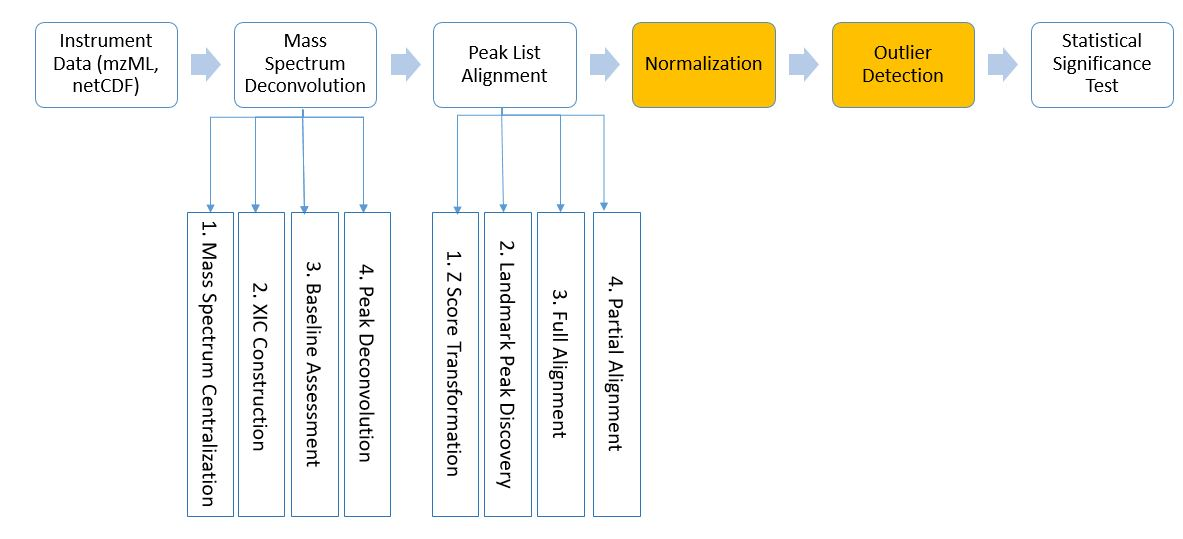
\includegraphics[width=16cm]{flow_data_process.JPG}
	\caption{Flowchart of LC-MS data analysis.}
	\label{flo}
\end{figure}

To calculate the area of a chromatographic peak from an XIC \cite{xic}, two approaches are usually used. The first approach sums all signals belonging to the chromatographic peak, while the other approach fits the chromatographic peak with a predefined peak model.\\
\indent The next component in the LC-MS data analysis is the peak list alignment \cite{lcms2}. The first step consists in applying z-score transformation to the retention time values to transform them into a normal distribution. This step is necessary to make the alignment of heterogenous experimental data possible mainly because experimental data is acquired under various experimental conditions.

For the actual alignment step, a peak list is selected as a reference and the rest of the
peak lists are aligned with respect to this reference. There are two steps of alignment; the full alignment followed by the partial alignment. The main purpose of full alignment is to identify
the landmark peaks, these are the set of metabolite peaks
generated by the same type of metabolites present in
every sample. In the partial alignment step, the peaks in a test sample
that are not recognized as the landmark peaks are aligned.\\
\indent To summarize, several analysis steps are involved in detecting molecular peaks from massive LC-MS data. Noise can be introduced at any of these steps. This noise is cumulated with the experimental errors to give highly noisy data. Thus, the next two components of LC-MS data analysis consist of data normalization and outlier detection. These two steps are required before analyzing the data and extracting information. 
Finally, an abundance test, such as the pairwise two-tail t-test, is performed on the normalized and cleaned peak areas to detect
the abundance changes of each metabolite between two sample
groups.

\section{Research Motivations} 
In proteomics and metabolomics, some analysis steps introduce technical variations that affect the peak areas of all molecules equally while others affect the peak areas of a subset of molecules with varying degrees. For instance, the inherent variability in the position of the syringe plunger position occurs whenever it is moved by the autosampler, which can easily introduce 2 \% variation in volume for all molecules (i.e. global technical variations). However, some data analysis algorithms have poor performance in deconvoluting overlapping chromatographic peaks, resulting in large variations in the peak areas of low abundance molecules (i.e. local technical variations). To correct these technical variations, existing normalization methods can only address the global technical variations. As a result, the local technical variations are ignored and may even be amplified in some cases.\\
While different normalization methods have been developed, these methods normalize the
abundances of all molecules detected in a sample based on certain assumptions \cite{clevland}\cite{astrand:eke}. However, these assumptions  usually do not hold for biological systems and may introduce biases in the normalized data.\\



The discovery of observations that deviates from normal behavior also known as outlier detection has
been widely studied in recent years \cite{outlier} \cite{outlier2}, resulting in a set of algorithms designed
to detect these rare but potentially crucial events. In some specific contexts an
outlier is a data point that can be considered either as an abnormality or noise.
The effect of undetected outliers in different application domains can have serious and disastrous
consequences. An example is the detection of landmines where an undetected
positive case implies an undetected landmine; another example is a failed attempt to
detect strange behavior in the use of a stolen credit card resulting in a financial
impact for the credit card holder. In both of these examples, the minority of the
cases represents the class of interest.

\section{Contributions}
 In this thesis, we focus on the two major steps highlighted in Figure \ref{flo} which are the normalization and outlier detection steps.
For outlier detection, the goal is to eliminate noisy undesired peaks.
We propose an algorithm that is based on the Fisher Criterion to detect the data points that lead to a remarkable change (whether increase or decrease) in the proposed criteria. The performance and robustness of the proposed method is validated using several experiments with real data sets.\\
\indent For the second contribution, we propose a molecule specific normalization algorithm, called MSN. MSN first identifies potential house-keepings, a group of molecules whose abundance levels were not affected by the biological treatment. MSN then adopts a robust surface fitting strategy to minimize the molecular profile difference of the house-keeping molecules across samples. Using different data sets, we compare our proposed MSN to several state-of-the-art normalization methods used for this application.

\indent The organization of the rest of this thesis is as follows. Chapter 2 provides a review of existing methods of normalization and outlier detection of omics data.
In chapter 3,  we  introduce our Fisher criterion based outlier detection and our molecule specific normalization and describe the different steps involved. In chapter 4, we describe the evaluation results of the proposed methods using our LC-MS metabolomics data set that motivated our approach, as well as the evaluation results using a publically available LC-MS proteomics data set. Then, we report the results of our experimental evaluations. Finally, we provide our concluding remarks and potential future work in chapter 5.
